../cictikz/src/cictikz/data/tex/cictikz_preamble.tex

% The trap's mean lifetime in the low state against inverse thermal
% energy, one point per chamber dwell. A straight line on this axis is an
% Arrhenius law, which is what identifies it as a trap in the silicon
% rather than as something in the instrument. Above about 55 degrees C the
% two levels merge into the noise and the fit stops meaning anything, so
% those dwells are left out.
%
% Generated by py/tikzplot.py. Edit the script in ex/ that
% produced it and re-run that, not this file.

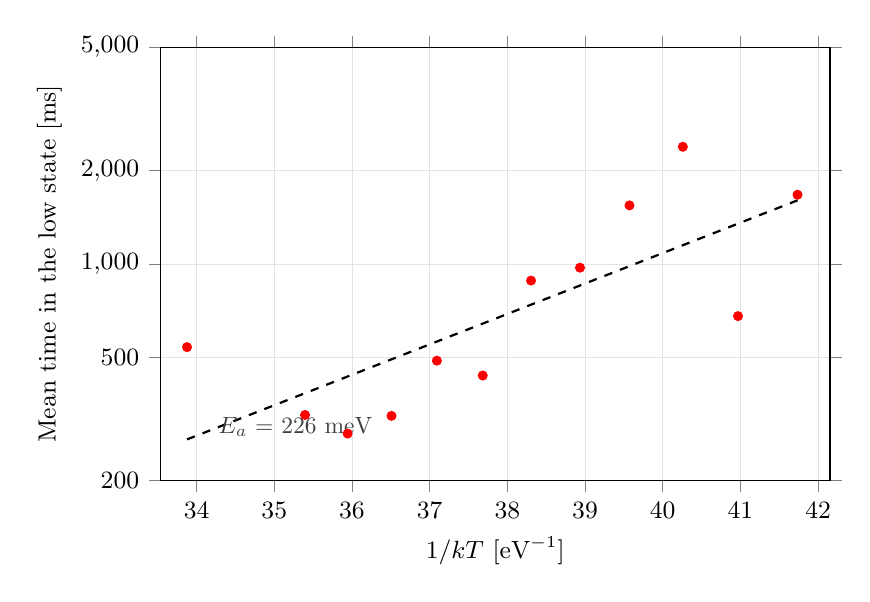
\begin{tikzpicture}[thick]

\begin{axis}[
  width=8.5cm,
  height=5.5cm,
  scale only axis,
  grid=both,
  grid style={gray!22, very thin},
  tick align=outside,
  tick label style={font=\small},
  label style={font=\small},
  title style={font=\small, yshift=-1mm},
  legend cell align=left,
  legend style={font=\small, draw=gray!50, fill=white, fill opacity=0.85, text opacity=1},
  ymode=log,
  xlabel={$1/kT$ [eV$^{-1}$]},
  ylabel={Mean time in the low state [ms]},
  xmin=33.538,
  xmax=42.153,
  ymin=200,
  ymax=5000,
  log ticks with fixed point,
  ytick={200,500,1000,2000,5000}
]
\addplot[red, only marks, mark=*, mark size=1.6pt, mark=none] coordinates {(41.735,1671.7) (40.969,678.1) (40.259,2387.8) (39.572,1544.5) (38.935,972) (38.305,883.2) (37.683,436.1) (37.093,486.9) (36.509,323.1) (35.944,283.2) (35.396,325.2) (33.877,538.5)};
\addplot[black, thick, dashed, mark=none] coordinates {(33.877,271.25) (41.735,1603.8)};
\node[anchor=south west, gray!50!black, scale=0.85, align=left] at (axis cs:34.177,260) {$E_a$ = 226 meV};
\end{axis}

\end{tikzpicture}
\end{document}
